\documentclass[a4 paper]{article}
% Set target color model to RGB
\usepackage[inner=2.0cm,outer=2.0cm,top=2.5cm,bottom=2.5cm]{geometry}
\usepackage{setspace}
\usepackage[rgb]{xcolor}
\usepackage{verbatim}
\usepackage{subcaption}
\usepackage{amsgen,amsmath,amstext,amsbsy,amsopn,tikz,amssymb,tkz-linknodes}
\usepackage{fancyhdr}
\usepackage[colorlinks=true, urlcolor=blue,  linkcolor=blue, citecolor=blue]{hyperref}
\usepackage[colorinlistoftodos]{todonotes}
\usepackage{rotating}
\usepackage{float}
% \usepackage{pgfplots}
%\usetikzlibrary{through,backgrounds}
\hypersetup{%
pdfauthor={Laxman,Pottimuthi,Sreeram Maddineni},%
pdftitle={Homework},%
pdfkeywords={Tikz,latex,bootstrap,uncertaintes},%
pdfcreator={PDFLaTeX},%
pdfproducer={PDFLaTeX},%
}
%\usetikzlibrary{shadows}
% \usepackage[francais]{babel}
\usepackage{booktabs}
\newcommand{\ra}[1]{\renewcommand{\arraystretch}{#1}}

\newtheorem{thm}{Theorem}[section]
\newtheorem{prop}[thm]{Proposition}
\newtheorem{lem}[thm]{Lemma}
\newtheorem{cor}[thm]{Corollary}
\newtheorem{defn}[thm]{Definition}
\newtheorem{rem}[thm]{Remark}
\numberwithin{equation}{section}

\newcommand{\homework}[8]{
   \pagestyle{myheadings}
   \thispagestyle{plain}
   \newpage
   \setcounter{page}{1}
   \noindent
   \begin{center}
   \framebox{
      \vbox{\vspace{2mm}
    \hbox to 6.28in { {\bf CS 520: Introduction to Artificial Intelligence \hfill {\small (#2)}} }
       \vspace{6mm}
       \hbox to 6.28in { {\Large \hfill #1  \hfill} }
       \vspace{6mm}
       \hbox to 6.28in { {\it Instructor: {\rm #3} \hfill Name: {\rm #5}, Netid: {\rm #6}} }
    %   \hbox to 6.28in { {\it TA: #4  \hfill #6}}
       \hbox to 6.28in { {\it TA: {\rm #4} \hfill Name: {\rm #7}, Netid: {\rm #8}} }
      \vspace{2mm}}
   }
   \end{center}
   \markboth{#6 / #8 -- #1}{#6 / #8-- #1}
   \vspace*{4mm}
}

\newcommand{\Question}[1]{~\\\fbox{\textbf{Question #1}}\newline}
\newcommand{\References}[1]{~\\\fbox{\textbf{REFERENCES #1}}\newline}
% \newcommand{\References}[1]{~\\\fbox{\textbf{References #1}\newline}
\newcommand{\subproblem}[1]{~\newline\textbf{(#1)}}
\newcommand{\D}{\mathcal{D}}
\newcommand{\Hy}{\mathcal{H}}
\newcommand{\VS}{\textrm{VS}}
\newcommand{\solution}{~\newline\textbf{\textit{(Solution)}} }

\newcommand{\bbF}{\mathbb{F}}
\newcommand{\bbX}{\mathbb{X}}
\newcommand{\bI}{\mathbf{I}}
\newcommand{\bX}{\mathbf{X}}
\newcommand{\bY}{\mathbf{Y}}
\newcommand{\bepsilon}{\boldsymbol{\epsilon}}
\newcommand{\balpha}{\boldsymbol{\alpha}}
\newcommand{\bbeta}{\boldsymbol{\beta}}
\newcommand{\0}{\mathbf{0}}


\begin{document}
\homework{Assignment \#1: Fast Trajectory Replanning}{Due: 02/25/20}{Abdeslam Boularias}{Aravind Sivaramakrishnan}{Laxman Pottimuthi}{lp642}{Sreeram Madineni}{sm2323}
\Question{0: Maze Creation}
\vspace{-15pt}
\begin{itemize}
    \item Maze was generated using a python library matplotlib
    \begin{figure}[H]
        \centering
        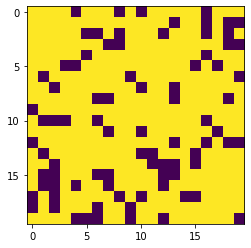
\includegraphics[scale=0.40]{sampleMaze.png}
        \caption{Sample Maze}
        \label{}
    \end{figure}
    \vspace{-20pt}
    \item According to requirement, maze was generated with 30\% probability that are marked. This can be seen in the method. Following is the code snippet:
    \begin{verbatim}
        def get_rand_value():
            rand_value = random.randint(0,9)
            if rand_value in [0,2]:
                return -1
            else:
                return 1
    \end{verbatim}
\end{itemize}
\vspace{-25pt}
\Question{1: Understanding Methods}

\textbf{\hspace{-15pt}Read the chapter in your textbook on uninformed and informed
(heuristic) search and then read the project description again. Make sure that you understand A* and the concepts of
admissible and consistent h-values.}

\subproblem{a} \textbf{Explain in your report why the first move of the agent for the example search problem from Figure 8 is to the east rather
than the north given that the agent does not know initially which cells are blocked.}\\

Agent first move towards east rather than north:
\begin{itemize}
    \item While calculating path, A* chooses optimal path based on the calculated f-value, where f = g + h.
    \item The cell on the east has an f value = 3 [1(g)+2(h)] and cell on the north has a f-value = 5 [1(g)+4(h)]
    \item Cell on the east will be chosen as it has least f value among both neighbors.
    \item As the cell doesn't know anything about the status of any blocked cells other than its neighbours it chooses to move in the east direction initially.
\end{itemize}
\subproblem{b} \textbf{This project argues that the agent is guaranteed to reach the target if it is not separated from it by blocked cells. Give a
convincing argument that the agent in finite gridworlds indeed either reaches the target or discovers that this is impossible
in finite time. Prove that the number of moves of the agent until it reaches the target or discovers that this is impossible is
bounded from above by the number of unblocked cells squared.}\\

Agent is guaranteed to reach the target if it is not separated from it by blocked cells. Reasons: 
\begin{itemize}
    \item Assume that there is a path from source to destination. Initially A* algorithm calculates the path from source to destination and the agent traverses along that path. If there is a blocked cell along the path then a fresh A* algorithm runs with the new starting point adjacent to the blocked cell. Then the path is computed and the agent traverses along the new path. This can go on until the agent reaches the destination. It cannot go in an infinite loop. The reason is as follows . Assume that there is a node n which has K paths to the destination. When the agent starts at node n it takes any of the k paths to the destination. If it is unable to reach the destination(due to a blocked cell) and if at any later point it reaches the node n then it takes any of the remaining k- 1 paths to the destination. It cannot take the path it traversed before as the agent remembers that there are blocked cells along that path , therefore its new path would be different. So the agent will traverse each path only once between a given source and destination. So it will keep traversing through every path between any starting cell and the destination until it reaches the destination.
    \item Assume that a path doesn't exist between the source and destination due to various blocked cells . There would a particular iteration in Repeated A* when the agent cannot compute the path from the source(which can be different than the starting source) to destination. During this iteration the open list becomes empty. This means there is no node left through which the agent can travel to destination. Then the program exits and the the agent is not able to destination.
    
    \item Assume that there are K unblocked nodes in the maze. Any of the K nodes can be starting point and each of the nodes can be a starting point of an A* iteration only once. This is true as the agent will be blocked at a node only once throughout its entire journey. It cannot be blocked at that node again as when it was blocked for the first time it will know about its neighbours and it will make sure to not blocked there again when it is computing path. So from each of the K nodes as starting points of A* algorithm the agent can make at most K moves (since the total number of unblocked nodes is K). So the total number of moves the agent makes in its entire journey has upper bound of K*K. SO the total number of moves it makes is O($K^2$)
\end{itemize}

\Question{2: The Effects of Ties}

\textbf{\hspace{-15pt}Repeated Forward A* needs to break ties to decide which cell to expand next if
several cells have the same smallest f-value. It can either break ties in favor of cells with smaller g-values or in favor of
cells with larger g-values. Implement and compare both versions of Repeated Forward A* with respect to their run time or,
equivalently, number of expanded cells. Explain your observations in detail, that is, explain what you observed and give a
reason for the observation}

\begin{itemize}
    \item Assume the tie breaks' are done using a priority, where priority = constant*f -/+ g. 
    \item If larger g-value tie break is used, then the priority is constant*f - g and if tie break is based on smaller g-value, priority is constant*f+g.
    \item If the tie break is based on larger g value, the cell is away from the starting point and if the g value is less, it means the cell is closer to start point.
    \item If the expanded cells are closer to the start point, we end up expanding non decreasing number of grid cells which are greater than when expanded a node cell from a cell away from the start point. 
    \item As the performance is dependent on number of expanded cells, expanding cells with greater g-value is considered for better performance.
    
    \begin{figure}[H]
        \centering
        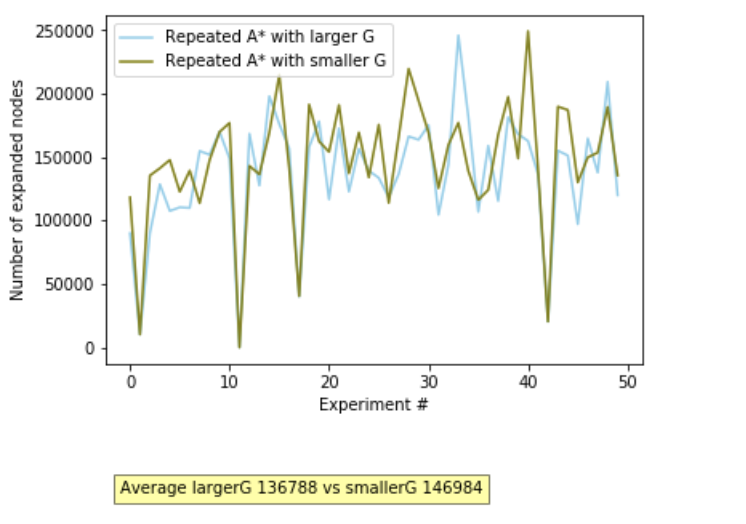
\includegraphics[scale=0.5]{smallerGvsLargerG.png}
        \caption{Repeated Forward $A^*$: Tie with larger G v smaller G}
        \label{Repeated Forward A^*: Tie with larger G v smaller G}
    \end{figure}

\end{itemize}

\Question{3: Forward vs. Backward}

\textbf{\hspace{-15pt}Implement and compare Repeated Forward A* and Repeated Backward A*
with respect to their runtime or, equivalently, number of expanded cells. Explain your observations in detail, that is, explain
what you observed and give a reason for the observation. Both versions of Repeated A* should break ties among cells with
the same f-value in favor of cells with larger g-values and remaining ties in an identical way, for example randomly.}

\begin{itemize}
    \item Repeated Backward A* expands more number of nodes and thus it runs slower than Repeated Forward A*.
    \item The reason is in the case of Repeated Backward A* the algorithm computes the path from destination to the source.
    \item But the agent knows more information(whether the cells are blocked or not) about the cells which are near the source and it has less information about cells which are near destination. So more cells near the destination are likely to be expanded while computing the path. 
    \item Also whenever the agent travels from the source to a blocked cell it only gathers information about the neighboring cells along the path, it is very unlikely that it would gather any information about cells which are near the destination. \item So this will cause unnecessary expansion of cells near the destination during path computation for every iteration of A*.
    
    \begin{figure}[H]
        \centering
        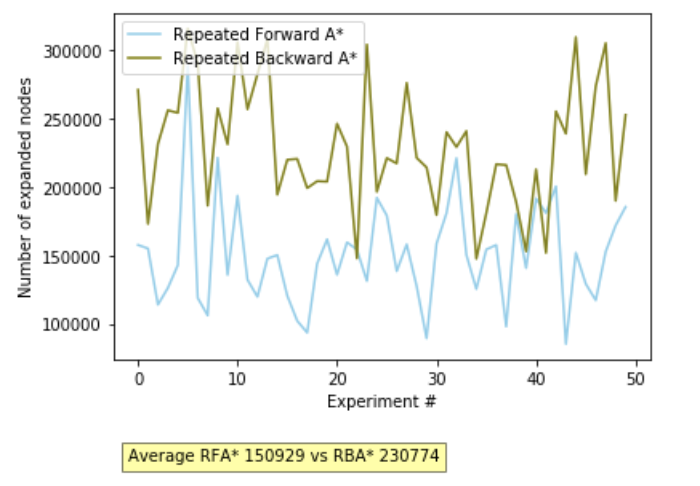
\includegraphics[scale=0.5]{rfa vs rba.png}
        \caption{Repeated Forward $A^*$ vs Repeated Backward $A^*$}
        \label{Repeated Forward A^* vs Repeated Backward A^*}
    \end{figure}
    
\end{itemize}

\newpage
\Question{4: Heuristics in the Adaptive A*: Consistent and admissible }

\textbf{\hspace{-16pt}The project argues that “the Manhattan distances are consistent in
gridworlds in which the agent can move only in the four main compass directions.” Prove that this is indeed the case.
Furthermore, it is argued that “The h-values $h_{new}$(s) ... are not only admissible but also consistent.” Prove that Adaptive A*
leaves initially consistent h-values consistent even if action costs can increase}


\textbf{\hspace{-15pt}a. Manhattan Distance consistent}
\begin{itemize}
    % \item To actually answer your question: the Manhattan distance is consistent when you're constrained to moving vertically/horizontally along an unweighted grid (this can be easily shown by the definition on Wikipedia). So yes, in your case you can avoid rechecking nodes in the closed set.
    
    % \item Manhattan distance is said to be consistent in the grid worlds when estimate is 
    \item h-values h(s) are consistent iff they satisfy the following triangle inequalities for all states s with s $\neq$ $s_{goal}$ and all actions a that can be executed in state s. \\
    \begin{equation}
    h(s_{goal}) = 0
    \end{equation}
    \begin{equation}
    h(s) \leq c(s, a) + h(succ(s, a))
    \label{eqn:forward}
    \end{equation}
    
    
    \begin{figure}[!htbp]
        \centering
        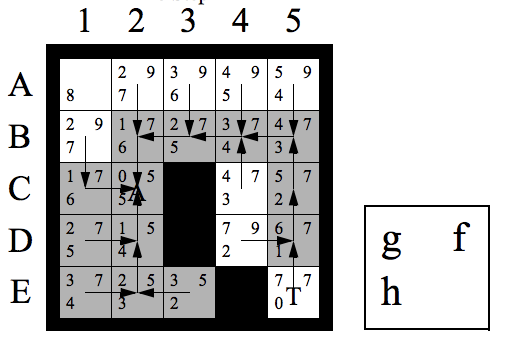
\includegraphics[scale=0.9]{Q4 pic.png}
        \caption{Forward A^*}
        \label{Forward A^*}
    \end{figure}
    
    \item Assume our goal is to move from A5 to E5. We do this by moving one step at a time with following pattern $A5 -> B5 -> C5  -> D5  -> E5.$ In the gridworld, movement can happen only in the four compass directions and the cost from moving from one gridcell to any immediate cell is same.
    \begin{equation}
    c(s, a) = c(s+1, a) = c(s+2,a)
    \end{equation}
    
    \item We can prove Manhattan distance is consistent using induction. From \ref{eqn:forward}, let us assume it is true for s, we will get the following
    \begin{equation}
    h(s) \leq c(s, a) + h(s+1)
    \label{eqn:ind_assumption}
    \end{equation}
     And we need to show this inequality holds for s+1
    \begin{equation}
    h(s+1) \leq c(s+1, a) + h(s+2)
    \label{eqn:ind_prove}
    \end{equation}  
    
    \item Cost of moving from s to s+1 is c(s,a) and cost of moving from s+1 to s+2 is c(s+1,a). In the gridworld Manhattan distance between two points is sum of unit distances.
    \item Let us assign coordinates to points to calculate distances. \\
    A5 - (i,j), B5 - (i, j+1), C5 - (i, j+2), E5 - (i, j+4)
    
    % \item Hence, \\
    % Distance from A5 to E5 is $h(s) = \sqrt{(i-i)^2+(j-j-4)^2} = 4$ \\
    % Distance from B5 to E5 is $h(s+1) = \sqrt{(i-i)^2+(j+1-j-4)^2} = 3$ \\
    % Distance from C5 to E5 is $h(s+2) = \sqrt{(i-i)^2+(j+2-j-4)^2} = 2$
    
    \item Hence, \\
    Distance from A5 to E5 is $h(s) = abs(i-i)+abs(j-j-4) = 4$ \\
    Distance from B5 to E5 is $h(s+1) = abs(i-i)+abs(j+1-j-4) = 3$ \\
    Distance from C5 to E5 is $h(s+2) = abs(i-i)+abs(j+2-j-4) = 2$
    
    \item From above, we can say \\
    \begin{center}
    h(s) = 1 + h(s+1) and h(s+1) = 1 + h(s+2) \\
    \end{center}
    From \ref {eqn:ind_assumption} \\
    \begin{center}
    $h(s) \leq c(s, a) + h(s+1)$ \\
    \implies 1 + h(s+1) \leq c(s, a) + 1 + h(s+2) \\
    \therefore h(s+1) \leq c(s+1, a) + h(s+2) \\
    \end{center}
    Hence proving \ref {eqn:ind_prove}, Manhattan distance consistency is proved by induction.
    
    
\end{itemize}

\textbf{\hspace{-15pt}b. The h-values $h_{new}$(s) ... are not only admissible but also consistent.}

\begin{itemize}
    \item It is mentioned that initially Manhattan distance is consistent. We need to prove that new h values are also consistent
    
    \item We have the below from how we calculate $h_{new}$ \\
    \begin{equation}
        h_{new}(s) = g(s_{goal}) - g(s)
    \end{equation}
    
    \begin{equation}
        h_{new}(s+1) = g(s_{goal}) - g(s+1)
    \end{equation} 

    \item Subtracting 0.6 from 0.7,
        \begin{center}
            $h_{new}(s) - h_{new}(s+1) = g(s_{goal}) - g(s) - (g(s_{goal}) - g(s+1))$ 
            $h_{new}(s) - h_{new}(s+1) = g(s_{goal}) - g(s) - g(s_{goal}) + g(s+1)$
        \end{center}
        \vspace{-10pt}
        \begin{equation}
            h_{new}(s) - h_{new}(s+1) = g(s_{goal}) - g(s_{goal}) + g(s + 1) - g(s)
        \end{equation}
    \item As s+1 and s are neighboring cells, 
        \begin{equation}
            g(s+1) - g(s) = 1
        \end{equation}
    \item Substituting 0.9 in 0.8,
        \begin{equation}
            h_{new}(s) =  1 + h_{new}(s+1)
        \end{equation}
    \item In 0.10, it is of the form, 
        \begin{center}
            $h(s) \leq c(s, a) + h(s+1)$ \\
        \end{center}
    \item In the considered maze we assumed cost from s to s+1 is one. So c(s,a) = 1
    \item Therefore new Manhattan distance($h_{new}$ ) is also a consistent heuristic.
    
    % \begin{equation}
    % h_{new}(s) \eq f_ + h_{new}(succ(s, a))
    % \end{equation}
    
    
    % \item Consider $h_{new}$ has increased by value k once it encountered a blockage. Therefore, $h_{new}(s) = h(s) +k$ and 
    % $h_{new}(s+1) =  h(s+1) +k$
    % \item Assuming $h_{new}$ is consistent by induction 
    % \begin{center}
    % $f_{new}(s) - g_{new}(s)\leq c(s,a) + f_{new}(s+1) - g_{new}(s+1)$
    
    % $f_{new}(s) - f_{new}(s+1) + g_{new}(s+1) - g_{new}(s) \leq c(s,a) $
    
    % \end{center}
    
    % \item As we moved only a single step ahead from s to s+1 with $h_{new}$ values, $g_{new}(s+1) = g_{new}(s) + 1$. Also the f values remain consistent since g \& h values are compensated. Therefore, $f_{new}(s) = f_{new}(s+1).$
    % \item From \ref{eqn:forward}, in gridworlds with movements in only four compass directions; c(s,a) = 1. From above, $1\leq c(s,a)$ indeed is true.
    % \item Therefore from induction, assumption is true, hence new Manhattan distance is also consistent heuristic.

\end{itemize}


\newpage
\Question{5: Heuristics in the Adaptive A*}

\textbf{\hspace{-15pt}Implement and compare Repeated Forward A* and Adaptive A*
with respect to their run-time. Explain your observations in detail, that is, explain what you observed and give a reason for
the observation. Both search algorithms should break ties among cells with the same f-value in favor of cells with larger
g-values and remaining ties in an identical way, for example randomly.}

\begin{itemize}
    \item On an average, Adaptive A* is much more efficient than A*. 
    \item 50 different experiments are tested for both the algorithms under similar conditions, i.e, maze, start and goal. 
    \item Performance of the algorithms are calculated by number of expanded nodes in each algorithm and averaging in the sample data.
    \item If the number of nodes expanded are less, it means algorithm performed better. 
    \item The result of the sample experiments: the average number of nodes expanded for Adaptive A* is 134181 nodes and of repeated forward A* is 140608 nodes.
    \item Adaptive A* on average is better than Repeated forward A*
    \item This performance difference is due to updating the h-value of previous iteration's expanded nodes in the current iteration.
    \item Adaptive A* h-value heuristic for the cells is a much better estimate of distance to the destination when compared to Forward A*. 
    \item While calculating the heuristic in the case of Forward A*( is Manhattan distance and ) it doesn't take data about blocked cells into consideration(since it doesn't not have it) to update the heuristic of any cell. 
    \item But Adaptive A* updates the heuristic function of every expanded cell in a particular iteration and use these heuristic values in the next iteration. 
    \item These new heuristic values give a better estimate of distance to destination leading to less number of expanded nodes.

    \begin{figure}[H]
        \centering
        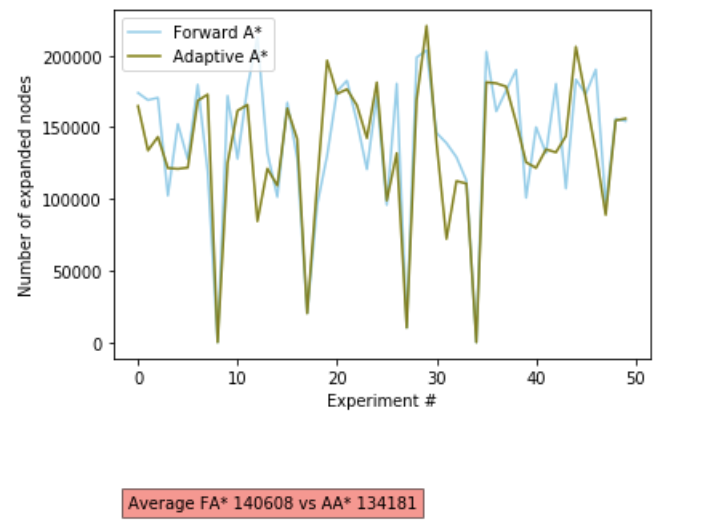
\includegraphics[scale=0.5]{fa vs aa.png}
        \caption{Adaptive $A^*$ vs Forward Repeated $A^*$ }
        \label{Adaptive A^* vs Forward Repeated A^*}
    \end{figure}
    
\end{itemize}

\newpage
\Question{6: Statistical Significance}

\textbf 
{ \hspace{-21pt} Performance differences between two search algorithms can be systematic
in nature or only due to sampling noise (= bias exhibited by the selected test cases since the number of test cases is always
limited). One can use statistical hypothesis tests to determine whether they are systematic in nature. Read up on statistical
hypothesis tests (for example, in Cohen, Empirical Methods for Artificial Intelligence, MIT Press, 1995) and then describe
for one of the experimental questions above exactly how a statistical hypothesis test could be performed. You do not need
to implement anything for this question, you should only precisely describe how such a test could be performed.}


\begin{itemize}
    \item The following is the procedure to determine the statistical significance of Repeated A* and Adaptive A* algorithms.
    % \vspace{-8pt}
    \item In order to perform, we need to choose a statistical hypothesis test to determine the statistical significance of the experiment. We can compare the performance difference of both the search algorithms based on number of expanded cells in the map.
    \item As we are considering two different experiments with 50 random sample data set, two sample tests could be chosen. Different type of hypothesis test statistics such as t-test and z-test can be used to determine the two sample test.
    \item Considering T-test as example, two sample T-test is used validating the hypothesis. As a comparison between experiments are made, one tailed test is used to accept/reject the hypothesis.
    \item In the following, AA* is adaptive A* test sample and RA* is Repeated forward A* test sample.
    
    \begin{equation}
     H_0 : AA^* = RA^* 
    \end{equation}
    \begin{equation}
     H_1 : AA^* > RA^* 
    \end{equation}
    
    \begin{equation}
    T_{stat} = \frac{AA^* - RA^*}{\sigma_{AA^* - RA^*}}
    \end{equation}
    
    \begin{equation}
    \sigma_{AA^* - RA^*} = 
    \sqrt{\frac{({n_{AA^*}}-1)s_{AA^*}^2 + ({n_{RA^*}}-1)s_{RA^*}^2 }
    {{n_{AA^*}} + {n_{RA^*}} - 2} 
    ( \frac{1}{n_{AA^*}} + \frac{1}{n_{RA^*}} )}
    \end{equation}
    
    \begin{equation}
    df = n_{AA^*} + n_{RA^*} - 2
    \end{equation}
    
    where

    $H_0$:     Null Hypothesis - Both the experiments perform equally good  \\
    $H_1$:     Alternative Hypothesis - Adaptive A* gives better performance compared to Repeated A* \\
    $\sigma_{AA^* - RA^*}$:   Standard error of difference between AA* and $RA^*$ \\
    $s_{AA^*}$ : Standard error of Adaptive A* \\
    $s_{RA^*}$: Standard error of $RA^*$ \\
    $n_{AA^*}$ : No. of samples in first algorithm \\
    $n_{RA^*}$: No. of samples in second algorithm \\
    df        : Degrees of freedom 
   
    \item A confidence interval should be chosen to perform the test. Using the confidence interval, significance of the test is calculated. Based on the type of the t-test(In this case, it's a 1-tailed T-test as mentioned above), critical values are calculated from the T-test statistic table. 

    \item For example, test is conducted at 95\% confidence. Critical values are calculated based on the confidence level and degrees of freedom. If the $T_{stat}$ is greater than critical value, Null Hypothesis is rejected. Thus it can be confirmed that the alternative hypothesis is accepted with 95\% confidence. It means that AA* will be outperforming RA*. 
\end{itemize}

\newpage
\References{}
\begin{itemize}
    \item \href{https://www.cs.cmu.edu/~maxim/files/adaptastar_aamas05.pdf}{\textbf{Adaptive A* by Sven Koenig and Maxim Likhachev }}
    \item \href{https://en.wikipedia.org/wiki/Consistent_heuristic}{\textbf{Consistent heuristic }}
    \item \href{https://en.wikipedia.org/wiki/Admissible_heuristic}{\textbf{Admissible Heuristic}}
\end{itemize}

\end{document} 

% \newpage
% \problem{2: Decision Trees, Overfitting}{5+5+10+5+10+10=45}

% \subproblem{a}

% \subproblem{b} 

% \subproblem{c}

% \subproblem{d} 

% \includegraphics[width=0.5\textwidth]{example-image-a}

% \subproblem{e} 

% \includegraphics[width=0.5\textwidth]{example-image-b}

% \subproblem{f}

% 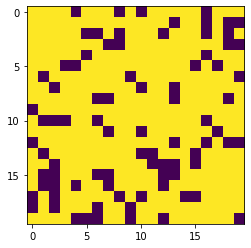
\includegraphics[width=0.5\textwidth]{sampleMaze.png}

% \newpage
% \problem{3: Hypothesis Testing}{15+10=25}
% \subproblem{a}

% \subproblem{b}

% \begin{table}[h]
% \centering
% \begin{tabular}{@{}lll|l@{}}
% \toprule
% \textit{Weather} & \textit{Food} & \textit{Meeting} & \textit{Attend?} \\ \midrule
% cold             & full          & idc              & yes              \\
% cold             & empty         & no               & no               \\
% hot              & full          & yes              & yes              \\
% cold             & full          & no               & yes              \\
% hot              & empty         & no               & no               \\ \bottomrule
% \end{tabular}
% \caption{Dataset $\D$\label{table:1}}
% \end{table}